\documentclass[11pt]{beamer}
\usepackage[utf8]{inputenc}
\usepackage[T1]{fontenc}
\usetheme{CambridgeUS}
\usepackage{xeCJK} 
\usepackage{graphics}
\usepackage{amssymb}
\setCJKmainfont{SimSun}
\begin{document}
\author{Changxu Miao}
\title[Math in FEM]{The Mathematic in Finite Element Method}
\subtitle{}
\institute{NWPU}
\date{\today}
\frame[plain]{\maketitle}

\begin{frame}{Outline}
\tableofcontents %[pausesections]
\end{frame}

\section{Analytical Description}
\subsection{Overall}
\begin{frame}{Analytical Description}
\begin{figure}
\centering
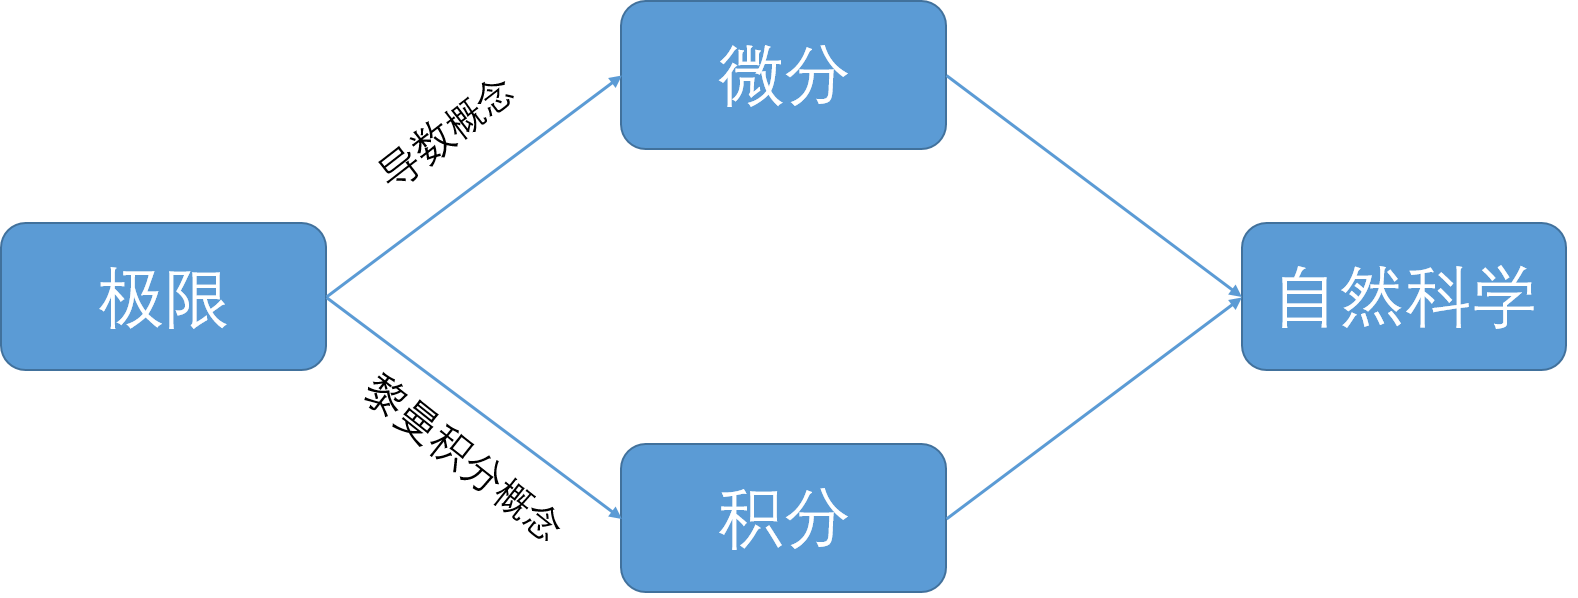
\includegraphics[width=0.9\linewidth]{source/zongshu}
\end{figure}
\end{frame}

\subsection{Differential}
\begin{frame}{Finite Difference Method}
\begin{figure}
\centering
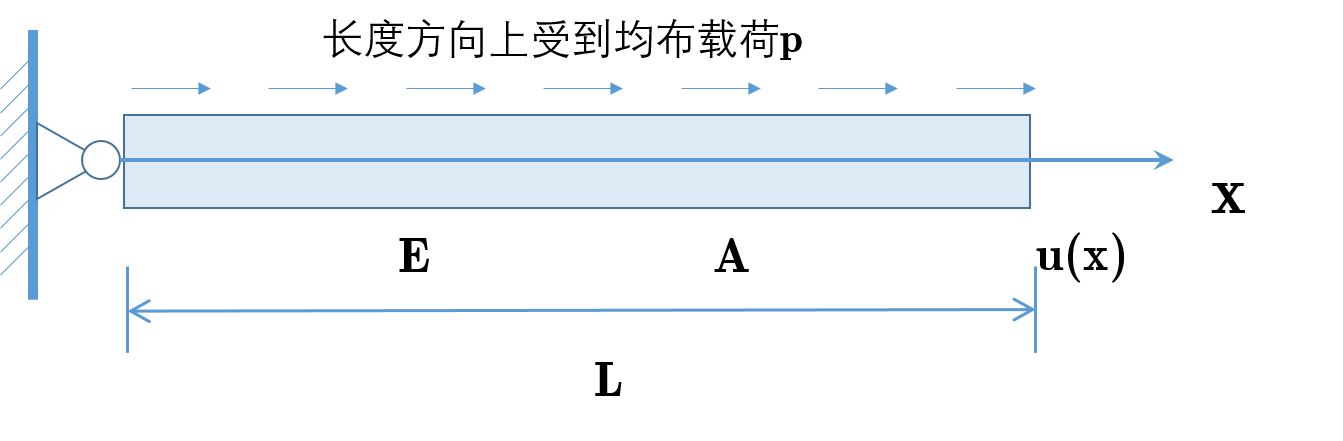
\includegraphics[width=0.7\linewidth]{source/differential}
\end{figure}
\begin{block}{Mathematical Description}
\begin{align*}
\frac{\mathrm{d}^2u}{\mathrm{d}x^2}+\frac{p}{AE}=0\quad\text{\color{red}(why?)}\\
\begin{cases}
u|_{x=0}=0 \quad\text{left end fixed}\\
\frac{\mathrm{d}u}{\mathrm{d}x}|_{x=L}=0\quad\text{right end free}
\end{cases}
\end{align*}
\end{block}
\end{frame}

\begin{frame}{Finite Difference Method}	
\begin{figure}
\centering
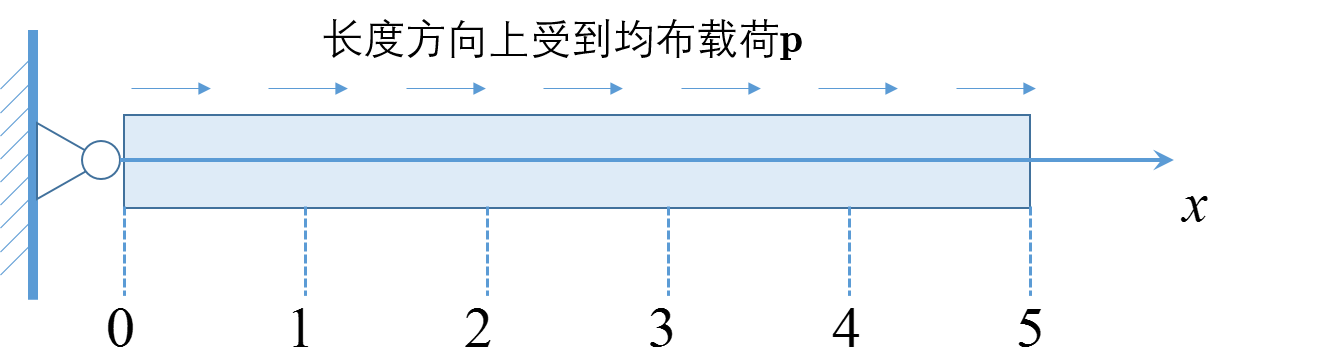
\includegraphics[width=0.7\linewidth]{source/differential_1}
\end{figure}

\begin{columns}
\column{0.36\textwidth}
\begin{block}{Difference Scheme}
\begin{align*}
\frac{u_{i-1}-2u_{i}+u_{i+1}}{\Delta l^2}=\frac{\mathrm{d}^2u}{\mathrm{d}x^2}\\
\text{$i$=1,2,3,4}
\end{align*}
\end{block}
\column{0.6\textwidth}
\begin{block}{Equation System}
\begin{align*}
\begin{cases}
u_0-2u_1+u_2+\frac{1}{5^2}\frac{PL^2}{AE}=0\quad\text{node 1}\\
u_1-2u_2+u_3+\frac{1}{5^2}\frac{PL^2}{AE}=0\quad\text{node 2}\\
u_2-2u_3+u_4+\frac{1}{5^2}\frac{PL^2}{AE}=0\quad\text{node 3}\\
u_3-2u_4+u_5+\frac{1}{5^2}\frac{PL^2}{AE}=0\quad\text{node 4}\\
\end{cases}
\end{align*}
\end{block}
\end{columns}
\end{frame}

\begin{frame}{Finite Difference Method}	
\begin{figure}
\centering
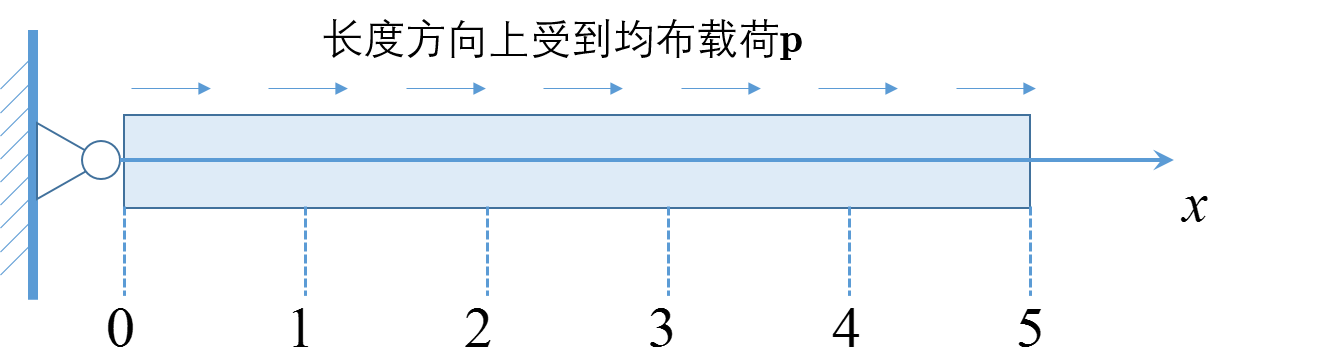
\includegraphics[width=0.7\linewidth]{source/differential_1}
\end{figure}

\begin{columns}
\column{0.2\textwidth}
\begin{block}{Boundary Condition}
\begin{align*}
u_0&=0\\
u_4&=u_5
\end{align*}
\end{block}
\column{0.75\textwidth}
\begin{block}{Equation System}
\begin{align*}
\left[ \begin{matrix}
-2&  1& 0 & 0 \\ 
1&  -2&1  &0  \\ 
0& 1 &  -2&1  \\ 
0& 0 & 1 & -2
\end{matrix}\right]
\left[
\begin{matrix}
u_1 \\ u_2\\u_3\\u_4
\end{matrix}  
\right] 
+
\frac{1}{5^2}\frac{PL^2}{AE}
\left[
\begin{matrix}
1 \\ 1\\1\\1
\end{matrix}  
\right] =0
\end{align*}
\end{block}
\end{columns}
\end{frame}


\subsection{Integral}
\begin{frame}{Galerkin Method}
\begin{block}{Mathematical Description}
\begin{align*}
&\frac{\mathrm{d}^2u}{\mathrm{d}x^2}+\frac{p}{AE}=0\\
&{\begin{cases}
u|_{x=0}=0 \quad\text{left end fixed}\\
\frac{\mathrm{d}u}{\mathrm{d}x}|_{x=L}=0\quad\text{right end free}
\end{cases}}
\end{align*}
\end{block}

\begin{block}{Process}
A trial function $\hat{u}_1(x)$ is selected to meet the BC, however, generally can not satisfy the governing equation. The deviation is evaluated by the residual function:
\begin{align*}
R=\frac{\mathrm{d}^2\hat{u}}{\mathrm{d}x^2}+\frac{p}{AE}-(\frac{\mathrm{d}^2u}{\mathrm{d}x^2}+\frac{p}{AE})=\frac{\mathrm{d}^2\hat{u}}{\mathrm{d}x^2}+\frac{p}{AE}
\end{align*}
\end{block}
\end{frame}

\begin{frame}{Galerkin Method}
\begin{example}
\begin{align*}
\hat{u}_1(x)=c_1\phi_1(x)=c_1sin\frac{\pi x}{2L}\\
\end{align*}
Solve the following integral equation and the coefficient $c_1$ will be obtained
\begin{align*}
\int\limits_{0}^{L}\phi_1R\mathrm{d}x=0
\end{align*}
\end{example}
\end{frame}


\begin{frame}{Galerkin Method}
\begin{example}
To improve the accuracy of approximate solution, another trial function is adopted.(can be explained by the fact that more terms of Fourier Series are used, the more they are close to the real function when a series of trigonometric functions are used to approach the rectangular wave)
\begin{align*}
\hat{u}_2(x)=c_1\phi_1(x)+c_2\phi_2(x)=c_1sin\frac{\pi}{2L}+c_2sin\frac{3\pi x}{2L}
\end{align*}

Solve the following integral equations and the coefficients $c_1$ and $c_2$will be obtained
\begin{align*}
\int\limits_{0}^{L}\phi_1R\mathrm{d}x=0,\quad\int\limits_{0}^{L}\phi_2R\mathrm{d}x=0
\end{align*}
\end{example}
\end{frame}


\begin{frame}{Galerkin Method}
\begin{example}
\begin{align*}
&\hat{u}_1(x)= \frac{16}{\pi^3}\frac{PL^2}{AE}sin\frac{\pi x}{2L}\\
&\hat{u}_2(x)= \frac{16}{\pi^3}\frac{PL^2}{AE}sin\frac{\pi x}{2L}+\frac{16}{27\pi^3}\frac{PL^2}{AE}sin\frac{3\pi x}{2L}\\
\end{align*}
\end{example}
\end{frame}

\subsection{Comparison}
\begin{frame}{Comparison}
\begin{figure}
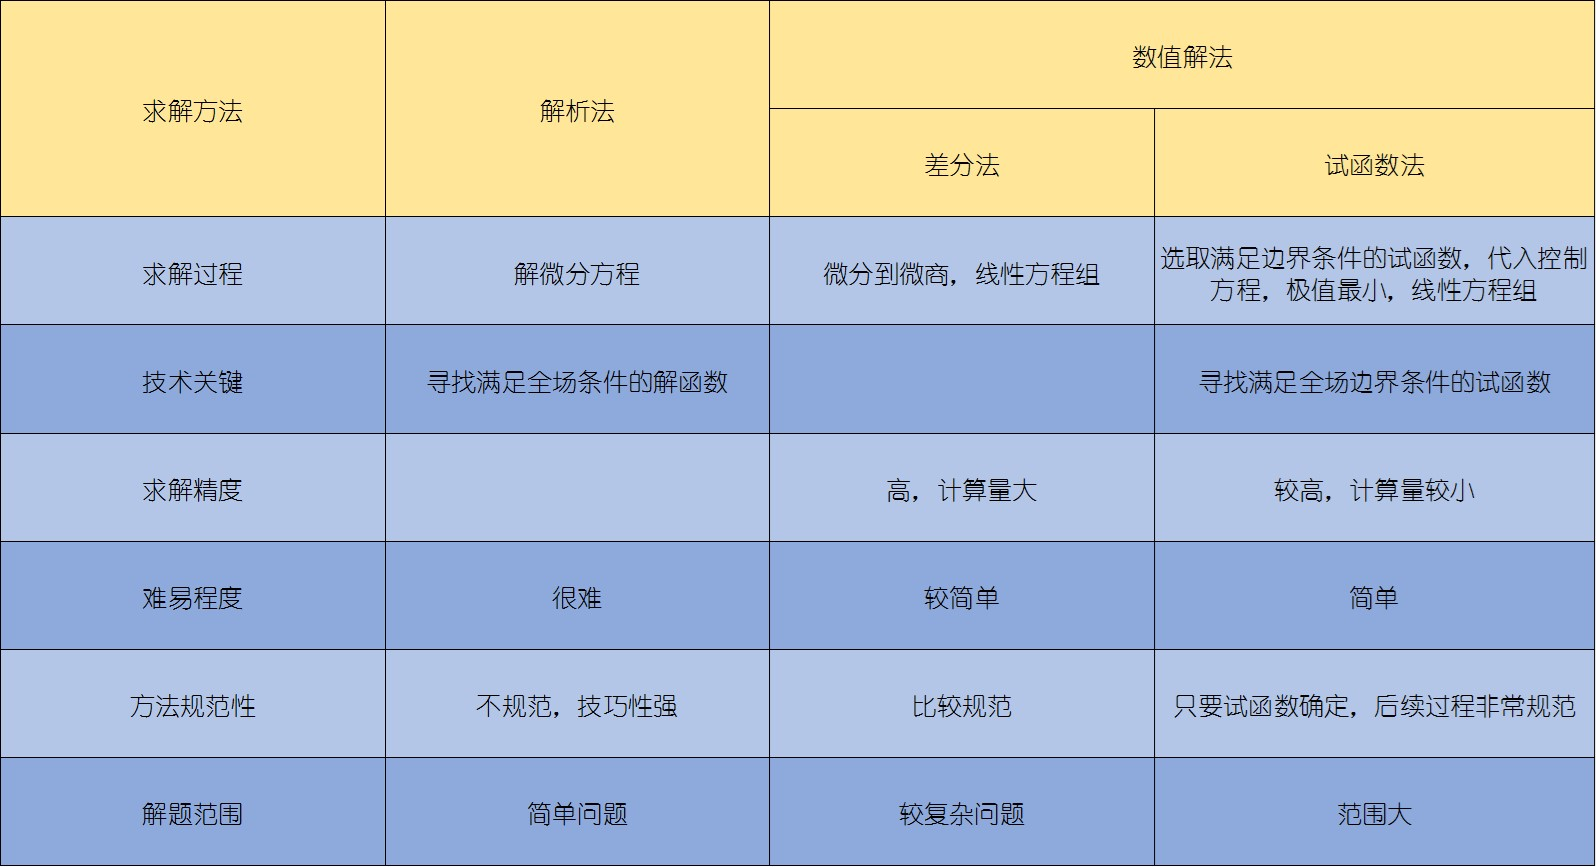
\includegraphics[width=1\linewidth]{source/bijiao}
\end{figure}\footnote{视频课程《有限元分析及应用》,清华大学,曾攀}
\end{frame}

\section{Comprehension}
\begin{frame}{Before the Beginning}
\begin{block}{Before the Beginning}
Both Ritz method and Galerkin method are the classical approaches to tackle the variational problem. They can be applied in derivation of basic equation in FEM, and respectively called Principle of Minimum Potential Energy and Principle of Virtual Work. Therefore, providing a novel way to solve partial equation system thereby avoiding solving on complex differential format.
\end{block}
\end{frame}

\subsection{Spring}
\begin{frame}{Principle of Minimum Potential Energy in spring}
\begin{columns}
\column{0.5\textwidth}
\begin{figure}
\centering
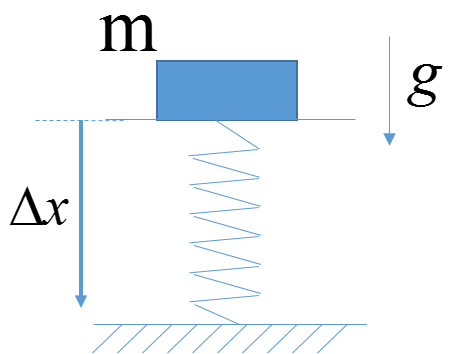
\includegraphics[width=0.6\linewidth]{source/spring}
\end{figure}
\column{0.5\textwidth}
\begin{block}{One of Nature' law}
Everything tends to stay in the comfortable zone, including humans.
\end{block}
\begin{block}{}
\begin{align*}
\Pi_p(\Delta x)&= \frac{1}{2}k\Delta x^2-mg\Delta x\\
\Pi_p'(\Delta x)&= k\Delta x-mg=0 \\
\Pi_p''(\Delta x)&= k>0
\end{align*}
\end{block}
\end{columns}
\begin{block}{Conclusion}
Only when $\Delta x = \frac{mg}{k}$, the system has minimum potential energy, simultaneously, is at static equilibrium.
\end{block}
\end{frame}

\subsection{Beam}
\begin{frame}{Principle of Minimum Potential Energy in one beam}
\begin{columns}
\column{0.5\textwidth}
\begin{figure}
\centering
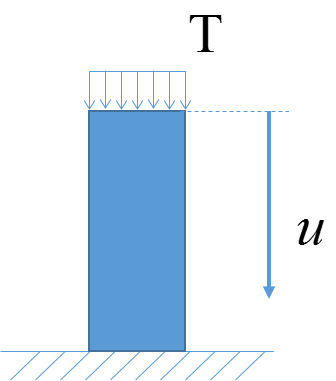
\includegraphics[width=0.6\linewidth]{source/simple_elastic_body}
\end{figure}
\column{0.5\textwidth}
\begin{block}{}
\begin{align*}
\Pi_p(u)&= \frac{EA}{2L}u^2-Tu\\
\Pi_p'(u)&= \frac{EA}{L}u-T \\
\Pi_p''(u)&= k>0
\end{align*}
\end{block}
\end{columns}
\end{frame}

\subsection{Beams}
\begin{frame}{Principle of Minimum Potential Energy in beams}
\begin{columns}
\column{0.5\textwidth}
\begin{figure}
\centering
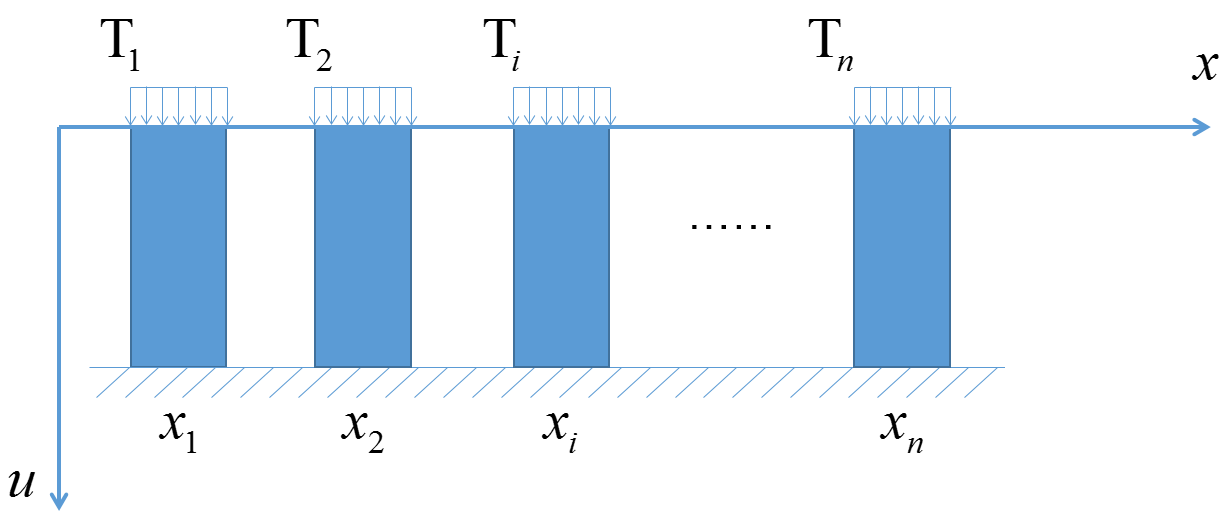
\includegraphics[width=1\linewidth]{source/many_elastc_body}
\end{figure}
\column{0.5\textwidth}
\begin{block}{}
\begin{align*}
\Pi_p(u)&= \sum\limits_{i=1}^{n} \frac{EA}{2L}u(x_i)^2-T(x_i)u(x_i)\\
\Pi_p'(u)&= \sum\limits_{i=1}^{n} \frac{EA}{L}u(x_i)-T\\
\Pi_p''(u)&= \sum\limits_{i=1}^{n} \frac{EA}{L}>0
\end{align*}
\end{block}
\end{columns}
\end{frame}

\subsection{Body}
\begin{frame}{Principle of Minimum Potential Energy in body}
\begin{columns}
\column{0.4\textwidth}
\begin{figure}
\centering
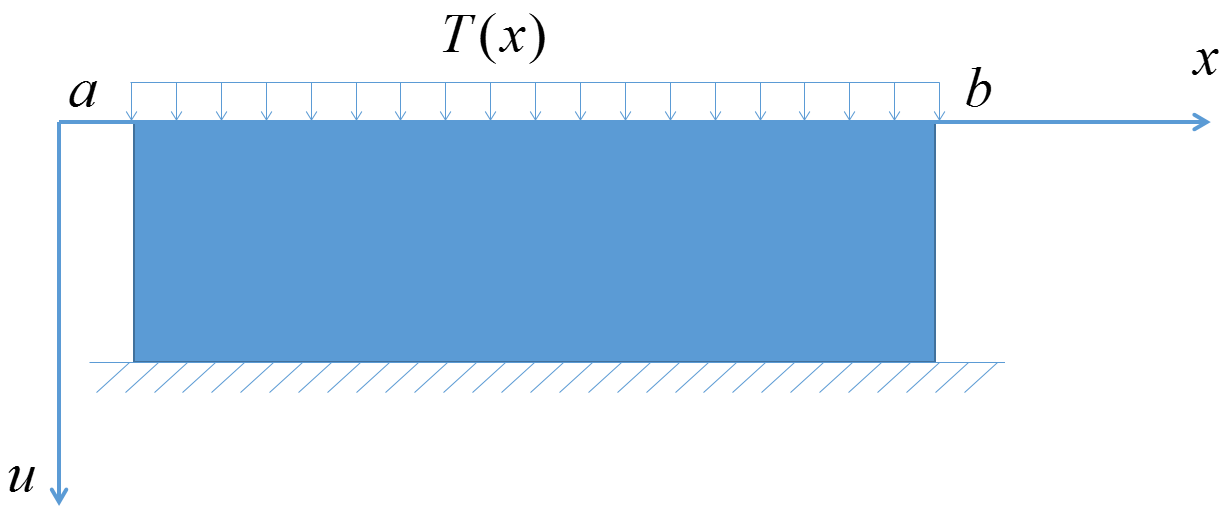
\includegraphics[width=1\linewidth]{source/continuous_elastc_body}
\end{figure}
\column{0.6\textwidth}
\begin{block}{}
\begin{align*}
\Pi_p(u)&=  \int\limits_{a}^{b}\frac{EA}{2L}u(x)^2-T(x)u(x)\mathrm{d}x\\
\delta\Pi_p(u)&= \int\limits_{a}^{b}\frac{EA}{L}u(x)\delta u(x)-T(x)\delta u(x)\mathrm{d}x\\
\delta^2\Pi_p(u)&= \int\limits_{a}^{b}\frac{EA}{L}\delta u(x)^2\mathrm{d}x>0
\end{align*}
\end{block}
\end{columns}
\end{frame}

\section{Principle of Minimum Potential Energy in Solid Mechanic}
\subsection{Reviews}
\begin{frame}{Basic equations}
\begin{block}{Basic equations}
\begin{description}
\item[Equilibrium equation:] $\sigma_{ij,j}+\overline{f_i}=0(\rho u_{i,tt})\qquad P\in\Omega$
\item[Geometric equation:] $\varepsilon_{ij}=\frac{1}{2}(u_{i,j}+u_{j,i})\qquad P\in\Omega$
\item[Constitutive equation:] $\sigma_{ij}=D_{ijkl}\varepsilon_{kl}\qquad P\in\Omega$
\item[Deformation compatibility equation:] $\varepsilon_{ij,kl}+\varepsilon_{kl,ij}=\varepsilon_{ik,jl}+\varepsilon_{jl,ik}$
\end{description}
\end{block}
\begin{block}{Boundary conditions}
\begin{description}
\item[Force:] $T_i = \overline{T_i}\qquad P\in\partial\Omega \quad\text{where}\quad T_i = \sigma_{ij}n_j$
\item[Displacement:]$u_i = \overline{u_i}\qquad P\in\partial\Omega$
\end{description}
\end{block}
\end{frame}


\begin{frame}{Basic equation}
\begin{block}{Energy}
\begin{description}   
\item[Strain energy]$U(\varepsilon_{mn})=\frac{1}{2}D_{ijkl}\varepsilon_{ij}\varepsilon_{kl}$
\item[Complementary energy] $V(\sigma_{mn})=\frac{1}{2}C_{ijkl}\sigma_{ij}\sigma_{kl}$   
\end{description}
\end{block}
\begin{figure}
\centering
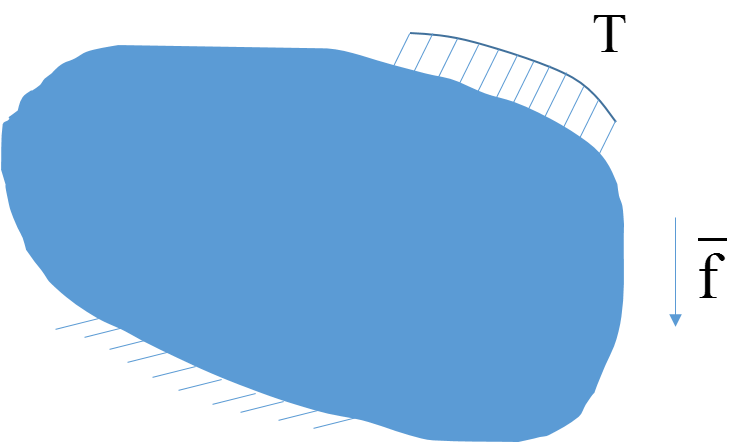
\includegraphics[width=0.7\linewidth]{source/general_elastic_body}
\end{figure}
\end{frame}

\subsection{Derivation}
\begin{frame}{Natural Variational Principle}
\begin{align}
\Pi_p(u_i)&=\int_\Omega\frac{1}{2}D_{ijkl}\varepsilon_{ij}\varepsilon_{kl}\mathrm{d}V-\int_{\partial\Omega}\overline{T_i}u_i\mathrm{d}S-\int_\Omega\overline{f_i}u_i\mathrm{d}V
\\
\delta\Pi_p(u_i)&=\int_\Omega D_{ijkl}\varepsilon_{kl}\delta\varepsilon_{ij}\mathrm{d}V-\int_{\partial\Omega}\overline{T_i}\delta u_i\mathrm{d}S-\int_\Omega\overline{f_i}\delta u_i\mathrm{d}V
\\
&=\underline{\int_\Omega\sigma_{ij}\delta\varepsilon_{ij}\mathrm{d}V}-\int_{\partial\Omega}\overline{T_i}\delta u_i\mathrm{d}S-\int_\Omega\overline{f_i}\delta u_i\mathrm{d}V
\end{align}
\end{frame}

\begin{frame}{Natural Variational Principle}
\begin{align}    
&\because\nonumber{\text{Geometric equation}}\quad \varepsilon_{ij}=\frac{1}{2}(u_{i,j}+u_{j,i})\qquad P\in\Omega
\\
&\therefore\int_{\Omega}\sigma_{ij}\delta \varepsilon_{ij}\mathrm{d}V
=\int_{\Omega}\frac{1}{2}\sigma_{ij}\delta (u_{j,i}+u_{i,j})\mathrm{d}V
\\
&\because \sigma_{ij} = \sigma_{ji}
\\
&\therefore \int_{\Omega}\sigma_{ij}\delta \varepsilon_{ij}\mathrm{d}V
=\int_{\Omega}\sigma_{ij}\delta u_{i,j}\mathrm{d}V
\\
&\because \nonumber{\text{Guass-Green formula:}}\quad \nabla(uv) = v \nabla u + u \nabla v
\\
&\therefore \int_{\Omega}\nabla(uv)\mathrm{d}V = \int_{\partial\Omega}uv\mathrm{d}\overrightarrow{S} = \int_{\Omega}\left(v \nabla u + u \nabla v\right)\mathrm{d}V
\\
&\int_{\Omega}\sigma_{ij}\frac{\partial\delta u_i}{\partial x_j} \mathrm{d}V = \int_{\partial\Omega}(\sigma_{ij}\delta u_i) n_j \mathrm{d}S -\int_{\Omega}\frac{\partial\sigma_{ij}}{\partial x_j}\delta u_i \mathrm{d}V
\end{align}
\end{frame}

\begin{frame}{Natural Variational Principle}
\begin{align}    
\delta \Pi &= \int_{\partial \Omega}\sigma_{ij}\delta u_i n_j \mathrm{d}S - \int_{\Omega}[\sigma_{ij,j}+\overline{f_i}]\delta u_i \mathrm{d}V - (\int_{sp}\overline{T_i}\delta u_i\mathrm{d}S+\int_{su}\overline{T_i}\delta u_i\mathrm{d}S)\\
&=\int_{\partial \Omega}\sigma_{ij}\delta u_i n_j \mathrm{d}S - \int_{\Omega}[\sigma_{ij,j}+\overline{f_i}]\delta u_i \mathrm{d}V - \int_{sp}\overline{T_i}\delta u_i\mathrm{d}S\\
&=\int_{sp}(\sigma_{ij}n_j-\overline{T_i})\delta u_i  \mathrm{d}S - \int_{\Omega}[\sigma_{ij,j}+\overline{f_i}]\delta u_i \mathrm{d}V
\end{align}
\end{frame}

\begin{frame}{Natural Variational Principle}
\begin{align}    
\delta^2 \Pi = \int_{\Omega}\frac{1}{2}D_{ijkl}(\delta\varepsilon_{ij})(\delta\varepsilon_{kl})\mathrm{d}V>0
\end{align}
\end{frame}

%\subsection{Principle of minimum complementary energy}
%\begin{frame}{Principle of minimum complementary energy}
%       
%\end{frame}

\begin{frame}{Natural Variational Principle}
\begin{align*}    
\Pi &= 
\int_{\Omega}\frac{1}{2}\{\varepsilon\}^T [D] \{\varepsilon\}\mathrm{d}S-
\int_{\Omega}\{u\}^T \{f\}\mathrm{d}V-\int_{s_\sigma} \{u\}^T \{T\}\mathrm{d}V\\
&= \int_{\Omega}\frac{1}{2}\{u\}^T[\partial]^T[D][\partial]\{u\}\mathrm{d}V-
\int_{\Omega}\{u\}^T \{f\}\mathrm{d}V-\int_{s_\sigma} \{u\}^T \{T\}\mathrm{d}S\\
&= \int_{\Omega}\frac{1}{2}\{q_e\}^T[N]^T[\partial]^T[D][\partial][N]\{q_e\}\mathrm{d}V-
\int_{\Omega}\{q_e\}^T[N]^T \{f\}\mathrm{d}V\\&-\int_{s_\sigma} \{q_e\}^T[N]^T \{T\}\mathrm{d}S\\
&= \frac{1}{2}\{q_e\}^T \left(\int_{\Omega} [N]^T[\partial]^T[D][\partial][N]\mathrm{d}V\right)\{q_e\}-\\&
\{q_e\}^T\left(\int_{\Omega}[N]^T \{f\}\mathrm{d}V-\int_{s_\sigma}[N]^T\{T\}\mathrm{d}S\right)
\end{align*}
thus get $[K]$ by comparing with $\Pi_p(\Delta x)= \frac{1}{2}k\Delta x^2-T\Delta x$
\end{frame}

\section{Differences in FEM, FDM, Ritz Method}
\begin{frame}
\begin{block}{有限差分法,Ritz法,有限元法的区别和联系}
有限差分法将问题的基本微分方程转化为差分方程或差分方程组,从而将求解微分方程的问题转化为求解线性代数方程组的问题。所得结果仅为在离散点上对真实结果的近似。

Ritz法利用系列试探函数的线性组合,利用能量泛函的驻值条件来确定线性组合系数。所得结果为在整个求解域上对真实结果的近似。这类方法在几何形状复杂问题上有一定局限性。

有限元法的单元离散思想借鉴于差分法,这使得有限元法在处理有复杂几何形状、复杂边界条件以及具有如圆孔应力集中等局部特征较强的问题上表现出优越性。

在小单元上的求解思想借鉴了Ritz法,这使得在子域中不用考虑整个求解域上的复杂边界条件且便于在同一求解域上使用不同单元类型。
\end{block}
\end{frame}
%
%\section{Constrained Variational Principles(广义变分原理)}
%\subsection{H-W Variational Principles(胡海昌-鹫津久广义变分原理)}
%\begin{frame}{H-W Variational Principles(胡海昌-鹫津久广义变分原理)}
%
%\end{frame}
%\subsection{H-R Variational Principles(Hellinger-Reissner变分原理)}
%\begin{frame}{H-R Variational Principles(Hellinger-Reissner变分原理)}
%
%\end{frame}

\end{document}